\documentclass[pdftex,10pt,a4paper]{article}
\usepackage{hyperref}
\usepackage{listings}
\usepackage{xyling}
\usepackage{ctable}

\input xy
\xyoption{all}

\begin{document}

  \title{SQL Windowing Functions with Hive\footnote{\copyright Copyright SAP AG 2011}}
  \author{Harish Butani \\
  \texttt{harish.butani@sap.com}}
  \maketitle

  \section{Overview}
This document describes a solution for issue (\cite{hive1}). Hive allows you to define UDFs, UDAFs and UDTFs. But none of these fit the model of Table-In/Table-Out functions needed to implement a generic solution. Hence we propose a solution that runs out of process from Hive and can be invoked as a Reduce script from Hive.  Admittedly this is far from an ideal solution: major performance issues in streaming  data back and forth; the functions are not integrated into Hive, hence the semantic layer doesn't get the complete picture of the processing, and also the data is sorted only in one way and not on a per function basis. But we think this is still an interesting exercise in extending Hive and hopefully the Windowing functions are useful on their own.

The overall flow of processing is shown in Figure \ref{arch}. Processing involves streaming data from a Hive Query/Table via the Script Operator:
\begin{figure}[h]
\centering
    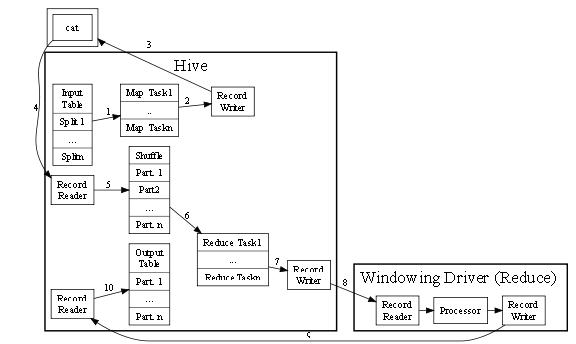
\includegraphics[scale=1]{architecture.jpg}
\caption{Overall processing of a Windowing Request}
\label{arch}
  \end{figure}
\begin{itemize}
\item The Map Operation is a Noop. It is used so that the M-R shuffle mechanism gets invoked for partitioning and sorting the input rows.
\item The {\em Readers} and {\em Writers}  capture the transformations that have to happen to integrate with an external process. The Windowing Process uses the TypedBytesSerDe for transforming bytes to Objects and back. The readers and writers handle the transformations from the input SerDe to TypedBytesSerDe and then to the output SerDe.
\item The Windowing Process is invoked during the Reduce phase. The Window process assumes that the data being streamed in is sorted. The Window process takes a {\em Windowing Query} that lists the operations to perform on the input stream.
\item The Output from the Windowing process is streamed back to the Script Operator. After going through the RecordReader it can then flow into the next operation in the Hive Query Graph.
\end{itemize}

The Windowing Processor is a generic Query Processor that can work in multiple modes. Conceptually it is fed a sorted input stream and a Windows Query that it generates a Output Stream that contains the results of the Windowing functions. Currently the Processor works in Hive mode and Local mode, with support for a MapReduce mode coming shortly. 
In Local mode instead of rows being streamed to the Processor, the Query specifies the Hive Table to process(actually the interface is at a lower level today, the user points to location, inputformat and serde details). The Query processing beyond how input is streamed is the same as Hive Mode. In MapReduce mode we will supporting generating a MR job to read an input location, stream it through the shuffle, and then run the Windowing Processor in the Reduce phase. Again apart from how input is brought to the Windowing Processor this mode works the same way as the other 2 modes.

In the following we describe the Window Query specification, and how the processor works. Finally we list some next steps.

  \section{The Windowing Query}
  Consider a sample Query:
  
    {\small
   \lstset{keywordstyle=\bfseries\underbar, emphstyle=\underbar,
     language=SQL, showspaces=false, showstringspaces=false}
   \begin{lstlisting}[caption={A sample Query},frame=shadowbox, numbers=left]
 from tableinput(
   recordreaderclass='windowing.io.TableWindowingInput',
   keyClass='org.apache.hadoop.io.Text', 
   valueClass='org.apache.hadoop.io.Text',
  inputPath='c:/Temp/partsmall',
  inputformatClass='org.apache.hadoop.mapred.TextInputFormat',
  serdeClass='org.apache.hadoop.hive.serde2.lazy.LazySimpleSerDe',
  columns = 'p_partkey,p_name,p_mfgr,p_brand,p_type,p_size,
                    p_container,p_retailprice,p_comment',
  'columns.types' = 'int,string,string,string,string,int,
                                string,double,string'
)
partition by p_mfgr
order by p_mfgr, p_name
with
  	rank() as r,
 	 sum(p_size) over rows between unbounded preceding 
 	                              and current row as s,
 	 ntile(<3>) as nt,
select p_mfgr,p_name, p_size, r, s, nt
   \end{lstlisting}
   }
  
  The Query form is:
  \begin{itemize}
  \item the {\em tableinput} clause specifies the input of the Query. In this case the storage details are specified; this is necessary when running in non hive mode. In all modes the Processor needs to be told the structure of the input; hence the 'columns' and 'column.types'  parameters are needed.
  \item the {\em partition} and {\em order by} clause specifies what columns the rows are ordered on and what are the partition boundaries. The order by columns must be a superset of the partition columns. Even though the ordering is not done by the Processor it needs to know about the ordering when doing ranking functions. The partition columns are used to divide the input into a set of partitions. The Window functions are applied on each Partition.
  \item Next the Query contains a list of function expressions. Currently there are 16 functions available. These are loosely  divided into Ranking, Aggregation and Navigation functions. Not all functions support a windowing clause. Functions are described by an annotation that specifies their details: name, description, windowing support, args with their names, types and if they are required/optional.
  \item The Processor uses Groovy for expression support. So arguments to functions can be columns, literals(strings, numbers or boolean) and also groovy expressions. Groovy expressions are enclosed in $<>$. For e.g. when requesting a {\em sum} one may write it as $sum(p\_size)$ which is saying compute the sum over the $p\_size$ column; but one can also write $sum(<p\_size/2>)$, which is a sum over the size divided by 2.
  \item The window clause supports both range boundaries and value boundaries. Boundaries can both start and end at Current Row.
  \item The Select List is a comma separated list of identifiers and/or groovy expressions. Groovy expression can be used to expressing ratios over computed aggregations.
  \item Not shown here is plans to support a where clause, which will support filtering out rows based on computed values.
  \end{itemize}
  
  
  Hive mode query looks very similar, except that the tableinput clause is much shorter:
  {\small
   \lstset{keywordstyle=\bfseries\underbar, emphstyle=\underbar,
     language=SQL, showspaces=false, showstringspaces=false}
   \begin{lstlisting}[caption={A Hive mode Query},frame=shadowbox, numbers=left]
from tableinput(
 columns = \'p_partkey,p_name,p_mfgr,p_brand,p_type,p_size,
                   p_container,p_retailprice,p_comment\',
 \'columns.types\' = \'int,string,string,string,string,int,
                              string,double,string\' )
 partition by p_mfgr 
 order by p_mfgr, p_name 
with 
 rank() as r, 
 sum(p_size) over rows between 2 preceding 
                    and 2 following as s, 
 min(<p_size>) over rows between 2 preceding 
                    and 2 following as m[int], 
 denserank() as dr, cumedist() as cud, 
 percentrank() as pr, 
 ntile(<3>) as nt, 
 count(<p_size>) as c, 
 count(<p_size>, \'all\') as ca, 
 count(<p_size>, \'distinct\') as cd, 
 avg(<p_size>) as avg, 
 stddev(p_size) as st, 
 first_value(p_size) as fv, 
 last_value(p_size) as lv, 
 first_value(p_size, \'true\') over rows between 2 preceding 
                                    and 2 following as fv2 
 select p_mfgr,p_name, p_size, r, s, m, dr, cud, pr, nt, c, 
          ca, cd, avg, st, fv,lv, fv2
   \end{lstlisting}
   }
  
   \begin{itemize}
   \item this Query lists more functions supported: denserank, percentrank, count (with all and distinct variations), stddev, $first\_value$, $last\_value$.
   \item In hive mode quotes must be escaped; this is because of handling by ScriptOperator and/or the shell. Additionally newlines may have to be removed. See below for a complete hive query.
   \item As mentioned before the details of the input don't need to be specified. In hive mode the Processor assumes the input stream is coming in from stdin and the format is TypedBytesSerDe.
   \end{itemize}
   
   The details of the language are beyond the scope of this doc; interested readers should look at the antlr grammar and the annotations for each function.
   
   \section{Details about the Processor}
   
   \subsection{Running the Processor}
   
   The processor takes 2 parameters: mode and query. Supported modes currently are local and hive, with mr coming shortly.
   In hive mode the Processor must be invoked from a Transform query. Here is a complete e.g.
   
{\small
   \lstset{keywordstyle=\bfseries\underbar, emphstyle=\underbar,
     language=SQL, showspaces=false, showstringspaces=false}
   \begin{lstlisting}[caption={A complete  Hive Query},frame=shadowbox, numbers=left]
CREATE TABLE windowing_test as
select p_mfgr,p_name, p_size, r, s, m, dr, cud, pr, nt, c, 
         ca, cd, avg, st, fv,lv, fv2
from
(
from (
  from part
  select transform(p_partkey,p_name,p_mfgr,p_brand,p_type,
                             p_size,p_container,p_retailprice,p_comment)
    ROW FORMAT SERDE 'org.apache.hadoop....TypedBytesSerDe'
    RECORDWRITER 'org.apache.hadoop.hive....TypedBytesRecordWriter'
    USING '/bin/cat'
    as (p_partkey,p_name,p_mfgr,p_brand,p_type,p_size,
         p_container,p_retailprice,p_comment)
    ROW FORMAT SERDE 'org.apache.hadoop...TypedBytesSerDe'
    RECORDREADER 'org.apache.hadoop....TypedBytesRecordReader'
    DISTRIBUTE BY p_mfgr
    SORT BY p_mfgr, p_name
) map_output
  select transform(p_partkey,p_name,p_mfgr,p_brand,p_type,
                p_size,p_container,p_retailprice,p_comment)
    ROW FORMAT SERDE 'org.apache.hadoop....TypedBytesSerDe'
    RECORDWRITER 'org.apache.hadoop....TypedBytesRecordWriter'
    USING 'java 
       -cp "antlr-runtime-3.4.jar:windowing.jar:groovy-all-1.8.0.jar...." 
       windowing.WindowingDriver 
       -m hive 
        -q "from tableinput(
        columns = \'p_partkey,p_name,p_mfgr,..\', 
        \'columns.types\' = \'int,string,string,...\' ) 
        partition by p_mfgr 
        order by p_mfgr, p_name 
        with
  	rank() as r,
 	 sum(p_size) over rows between unbounded preceding 
 	                              and current row as s,
 	 ntile(<3>) as nt,
select p_mfgr,p_name, p_size, r, s, nt"'
as (p_mfgr,p_name, p_size, r, s, nt)
ROW FORMAT SERDE 'org.apache.hadoop....TypedBytesSerDe'
RECORDREADER 'org.apache.hadoop....TypedBytesRecordReader'
) reduce_output;
   \end{lstlisting}
   }
   
\begin{itemize}
\item the map\_output part of the query is to stream the input data through the shuffle phase to do the partitioning and sorting.
\item the call to the WindowingProcessor is almost the same as in local mode.
\item To connect the pieces the RecordWriter and RecordReader with the TypedBytesSerDe must be specified in the Query.
\end{itemize}

\subsection{Processor internals}
\begin{figure}[h]
\centering
    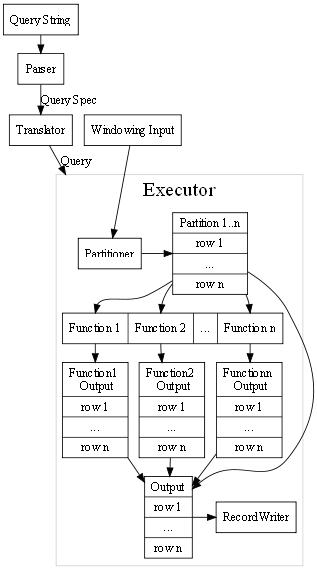
\includegraphics[scale=1]{query.jpg}
\caption{Execution of a Query}
\label{qry}
  \end{figure}
  The internal  flow of processing a Query  is shown in Figure \ref{qry}.
  \begin{itemize}
  \item A Query String is converted into a Query Object and passed to the Executor. A Query contains a list of Windowing Functions, the Windowing Input and an Output Writer.
  \item The executor streams the rows from the WindowingInput through the Partitioner. This produces a table for each Partition. It then passes the table to each Windowing Function which evaluates the function for the Partition ( and if necessary for a specific window for each row in the partition). The function outputs an Object that can be asked for results for each row row in the input.
  \item The Executor then creates an Output Object for each input row in the partition by processing the select list. The Output Object is then passed to the Output Writer.
  \item during execution the Functions and the Output processing have a GroovyShell at their disposal. When functions evaluate Groovy Expressions the columns of the Input are bound to the execution environment and can be used as variables. When the Output is processed both the input columns and the outputs of functions are available as variables.
  \item Not shown in this picture is the post filtering on Output Objects.
  \end{itemize}
    
\section{Summary}
\begin{enumerate}
\item As an analogy to Oracle, look at this as a quick implementation in PL/SQL. Typically new DB features are implemented in PL/SQL, once they show value they are pushed down into the Engine and finally integrated with the Semantic layers.
\item In this regard it would have been helpful if there was an In-Process Script Operator. This would avoid the overhead of streaming data to an external process.
\item The implementation hopefully shows a technique for providing extensible mini DSLs. We hope to use this pattern for introducing other Operations specifically for dimensional processing in OLAP.
\end{enumerate}

\section{Possible Next Steps}
\begin{description}
\item[Performance]  The data is going through several transformations: serialization through TypedBytesSerDe, inter process streaming, copy to a Standard Java Object, serialization through TypedBytesSerDe, and finally inter process streaming. Need to look at avoiding some of these conversions. Along these lines it would be nice to avoid streaming data through to an external process. Another performance improvement is on the evaluation of the Functions. 

Currently the Executor is very simple. It can be parallelized, and it can be made smarter when computing windows. Currently for computing windows the Executor computes the raw expressions for each row in the Partition in the first pass and then processes each row w.r.t. to its window range in a second pass. In this way it avoids computing the raw expressions multiple times, but it still takes $O(n^2)$  time.
\item[Metadata] The details about the input need to be specified in the Query. This can easily be improved to have the Windowing Processor read these details from the Metadata server.
\item[Map Reduce mode]  This would make the Windowing Processor usable as a standalone component.
\item[Multiple Orderings] since we use MR shuffle to do the sorting and partitioning we are restricted to a single Ordering and Partitioning; whereas in SQL each function can have its own ordering and partitioning.  This is a hard limitation to remove, but we can go halfway by allowing for multiple orderings within each partition. 

We could allow for secondary orderings for rows within a partition. The input would still come in sorted as now based on a primary ordering. The Partitioner can be extended to sort rows in a partition based on secondary sorting specifications and feed this ordering of rows into windowing functions.
\end{description}
  
  \begin{thebibliography}{Dillon 83}
   \bibitem[Hadoop]{hdop} Hadoop website {\em http://tiny.cc/b72fb}
   \bibitem[Hive]{hive} Hive website {\em http://tiny.cc/559sh}
   \bibitem[Hive ICDE]{hv10} Hive - A Petabyte Scale Data Warehouse Using Hadoop {\em http://tiny.cc/o5q6h}
   \bibitem[Hive 896]{hive1} Hive Issue 896 {\em https://issues.apache.org/jira/browse/HIVE-896}
  \end{thebibliography}
\end{document}
